\title{CS313, Lab - 2} % You may change the title if you want.
% \subtitle{Hello}
\author{Rishit Saiya, 180010027}

\date{\today}

\documentclass[12pt]{article}
\usepackage{fullpage}
\usepackage{enumitem}
\usepackage{amsmath,mathtools}
\usepackage{amssymb}
\usepackage[super]{nth}
\usepackage{textcomp}
\usepackage{hyperref}
\hypersetup{
    colorlinks=true,
    linkcolor=blue,
    filecolor=magenta,      
    urlcolor=cyan,
}
\begin{document}
\maketitle

%---------------------------------------------------------------------

\section{}

\begin{enumerate}
    \item \textbf{\textit{Student: Zhang's Profile:}} \\
    Student Name: Zhang \\
    Student ID: 00128 \\
    Department Name: Comp. Sci. \\
    Courses Taken: CS101, CS347 \\
    Course Names: CS101 $\rightarrow{}$ Intro. to Computer Science , CS347 $\rightarrow{}$ Database System  Concepts\\
    Grades: CS101 $\rightarrow{}$ A, CS347 $\rightarrow{}$ A- \\
    Credits: CS101 $\rightarrow{}$ 4, CS347 $\rightarrow{}$ 3 \\
    Instructors Names: CS101 $\rightarrow{}$ Srinivasan, Katz, Brandt \& CS347 $\rightarrow{}$ Srinivasan, Katz, Brandt \\
    Year: 2017 \\
    Semester: Fall \\
    Section ID: 1 \\
    Total Credits: 102 \\
    Advisor: Katz \\
    Building: Taylor \\
    Budget: 100000 \\
    
    The following queries were executed to get above information: \\
\begin{verbatim}
    select * from student natural join takes
    select * from student natural join department
    select * from student natural join classroom
    select * from student natural join course
    select * from department natural join instructor
    select * from course natural join instructor
\end{verbatim}


Alternatively, the query can be optimized as follows:
\begin{verbatim}
    select * from student,department,takes,advisor,instructor where
    student.name = 'Zhang' and advisor.s_ID = student.ID and student.ID =
    takes.ID and department.dept_name = student.dept_name and
    instructor.ID = advisor.i_ID
\end{verbatim}

The table is very long and couldn't be attached here.

\item I executed this query and got the following output.
\begin{verbatim}
    select title, course_id from course where course_id in (select course_id from
    instructor natural join teaches where ID = (select ID from instructor where
    name = 'Srinivasan'))
\end{verbatim}

Figure 1 shows the output to above query.
\begin{figure}
    \centering
    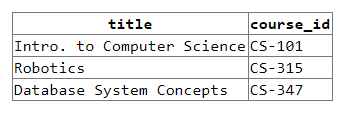
\includegraphics[width=12cm, height=4cm]{2.b.png}
    \caption{The id’s and titles of all courses taught by Instructor Srinivasan}
\end{figure}
    
\end{enumerate}


%---------------------------------------------------------------------
\end{document}